\chapter{Gestione dell'Input/Output}

\section{Dispositivi di I/O}
L'input/output è un'area assai problematica per la progettazione di sistemi operativi perché c'è una grande varietà di dispositivi di I/O e anche una grande varietà di applicazioni che li usano, per questo motivo è difficile scrivere un sistema operativo che tenga conto di tutte queste diversità. Possiamo dividere i dispositivi di I/O in tre categorie: 
\begin{itemize}
    \item i dispositivi \textit{leggibili dall'utente} che sono usati per la comunicazione diretta con l'utente, come stampanti, monitor, tastiera, mouse...
    \item i dispositivi \textit{leggibili dalla macchina} sono usati per la comunicazione con materiale elettronico, come dischi, chiavi USB, sensori, controllori, attuatori...
    \item i \textit{dispositivi di comunicazione} sono usati per la comunicazione con dispositivi remoti, come modem, schede Ethernet, Wi-Fi...
\end{itemize}

Un dispositivo di input prevede di essere interrogato sul valore di una certa grandezza fisica al suo interno. Ad esempio in una tastiera troviamo il codice Unicode degli ultimi tasti premuti, in un mouse le coordinate dell'ultimo spostamento effettuato, su disco il valore dei bit che si trovano in una certa posizione al suo interno. Un processo che effettua una syscall \verb|read| su un dispositivo del genere vuole conoscere questo dato per poterlo elaborare.

Un dispositivo di output prevede di poter cambiare il valore di una certa grandezza fisica al suo interno. Ad esempio un monitor moderno cambia il valore RGB di tutti i suoi pixel, una stampante moderna ottiene un file PDF o PS da stampare, un disco cambia il valore dei bit che devono sovrascrivere quelli che si trovano in una certa posizione al suo interno. Un processo che effettua una syscall \verb|write| su un dispositivo del genere vuole cambiare qualcosa.

Ci sono quindi, principalmente, due syscall \verb|read| e \verb|write| e, tra i loro argomenti, c'è un identificativo del dispositivo da leggere o scrivere. Il kernel, che comanda l'inizializzazione del trasferimento di informazioni, mette il processo in Blocked e passa ad altro, questa parte del kernel che gestisce un particolare dispositivo di I/O è chiamata \textit{driver}. A trasferimento completato, si genera l'interrupt che termina l'operazione e il processo ritorna Ready.

I dispositivi di I/O possono differire sotto molti aspetti: 
\begin{itemize}
    \item \textit{data rate} indica la frequenza di accettazione/emissione di dati. Possono esserci differenze di diversi ordini di grandezza tra le velocità di trasferimento dati, la Figura \ref{fig:data-rate} fornisce alcuni esempi;

    \begin{figure}[h]
        \centering
        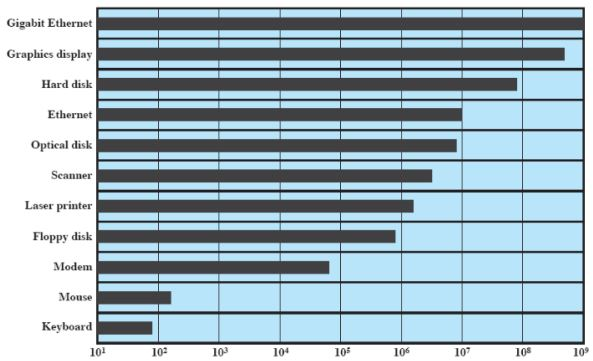
\includegraphics[width=0.7\linewidth]{images/data-rate.JPG}
        \caption{Data rate in bit per second}
        \label{fig:data-rate}
    \end{figure}

    \item l'\textit{applicazione} a cui viene destinato un dispositivo, ad esempio un disco utilizzato per i file richiede il supporto del software di gestione dei file, un disco utilizzato come archivio di backup per le pagine di memoria virtuale dipende dall'uso dell'hardware e del software della memoria virtuale. Oppure un terminale può essere utilizzato da un utente normale o da un amministratore di sistema, questi usi implicano diversi livelli di privilegio e forse diverse priorità nel sistema operativo;

    \item le \textit{difficoltà di controllo}, come in una stampante che richiede un'interfaccia di controllo relativamente semplice al contrario di un disco che è molto più complesso. L'effetto di queste differenze sul sistema operativo è filtrato in una certa misura dalla complessità del modulo I/O che controlla il dispositivo;

    \item l'\textit{unità di trasferimento dati} che trasferisce i dati dal dispositivo che li genera alla memoria o viceversa, come flusso di byte o in blocchi più grandi di dimensione fissa;

    \item la \textit{rappresentazione dei dati} in quanto i dati sono rappresentati secondo codifiche diverse in dispositivi diversi;

    \item le \textit{condizioni di errore} perché in base alla natura degli errori varia di molto dal tipo di dispositivo. Ad esempio varia nel modo in cui gli errori vengono notificati, sulle loro conseguenze (fatali/ignorabili) o su come possono essere gestiti.
    
\end{itemize}

\section{Organizzazione della funzione di I/O}
Come abbiamo visto nella Sezione \ref{sec:miglioramento-accessi}, le tecniche per gestire l'I/O sono: utilizzando la CPU, con o senza interruzioni, o utilizzando la memoria con il DMA.
Nell'ultimo caso, il processore delega le operazioni di I/O al modulo DMA, che trasferisce i dati direttamente da o verso la memoria principale. Quando l'operazione è completata, il modulo DMA genera un interrupt per il processore.

\subsection*{Evoluzione della funzione di I/O}
Nel corso degli anni la funzione di I/O ha subito notevoli migliorie che possono essere riassunte nei seguenti punti:
\begin{enumerate}
    \item Il processore controlla direttamente un dispositivo periferico;
  \item Viene aggiunto un modulo (o controllore) di I/O, direttamente sul dispositivo e il processore utilizza I/O programmato senza interruzioni;
  \item Vengono aggiunti gli interrupt in modo da migliorare l'efficienza del processore che non deve aspettare il completamento dell'operazione di I/O;
  \item Al modulo I/O viene dato il controllo diretto della memoria tramite DMA. Ora può spostare un blocco di dati da o verso la memoria senza coinvolgere il processore, tranne all'inizio e alla fine del trasferimento;
  \item Il modulo I/O è stato migliorato per diventare un processore separato (\textit{I/O channel}), con un set di istruzioni specializzate su misura per l'I/O. La CPU dirige il processore di I/O per eseguire un programma di I/O nella memoria principale. Il processore di I/O recupera ed esegue queste istruzioni senza l'intervento del processore. Ciò consente al processore di specificare una sequenza di attività I/O e di essere interrotto solo quando l'intera sequenza è stata completata;
  \item Il modulo I/O ha una propria memoria locale ed è, di fatto, un computer a sé stante (\textit{I/O processor}). Con questa architettura è possibile controllare un ampio insieme di dispositivi I/O, con un coinvolgimento minimo del processore. Un uso comune di tale architettura è stato quello di controllare le comunicazioni con terminali interattivi.
\end{enumerate}

\section{Problemi nel progetto del sistema operativo}
\subsection*{Obiettivi di progettazione}
Due obiettivi sono fondamentali nella progettazione della struttura di I/O: efficienza e generalità. L'\textit{efficienza} è importante perché la maggior parte dei dispositivi I/O sono estremamente lenti rispetto alla memoria principale e al processore. Un modo per affrontare questo problema è la multiprogrammazione che, come abbiamo visto, consente ad alcuni processi di attendere operazioni di I/O mentre un altro processo è in esecuzione, tuttavia spesso accade che l'I/O non tenga il passo con le attività del processore. E' necessario quindi cercare soluzioni software dedicate, a livello di sistema operativo, in particolare per l'I/O del disco.

Con la \textit{generalità} si vogliono gestire tutti i dispositivi in modo uniforme, per semplicità e per evitare errori. Ciò vale sia per il modo in cui i processi visualizzano i dispositivi I/O sia per il modo in cui il sistema operativo gestisce i dispositivi e le operazioni I/O. Ciò si può fare nascondendo la maggior parte dei dettagli dell'I/O del dispositivo nelle routine di livello inferiore in modo che i processi utente e i livelli superiori del sistema operativo vedano i dispositivi in termini di funzioni generali (lettura, scrittura, apertura, chiusura, blocco e sblocco).

\subsection*{Struttura logica della funzione I/O}
Con la progettazione gerarchica, le funzioni del sistema operativo vengono separate in base alla loro complessità, alla loro
scala temporale e al loro livello di astrazione. Seguendo questo approccio si arriva ad un'organizzazione del sistema operativo in una serie di livelli, dove ogni livello, si basa su quello inferiore per eseguire funzioni più primitive e fornisce servizi al livello superiore. La modifica dell'implementazione di un livello non dovrebbe avere effetti sugli altri livelli e, per l'I/O, ci sono 3  macro-tipi maggiormente usati:
\begin{itemize}
    \item Nel \textit{Dispositivo Locale}, il \verb|Logical I/O|: tratta il dispositivo come una risorsa logica per semplici operazioni (open, close, read, ...), il \verb|Device I/O|: trasforma richieste logiche in sequenze di comandi di I/O e lo \verb|Scheduling and Control|: esegue e controlla le sequenze di comandi (vedi Figura \ref{fig:struttura-funzione-io});
    \item Nel \textit{Dispositivo di Comunicazione} (scheda Ethernet, WiFi, ...), al posto del Logical I/O, c'è una \verb|Architettura di Comunicazione|, nella quale il dispositivo viene visto come una risorsa logica. A sua volta, questa consiste in un certo numero di livelli come vedremo nelle architetture TCP/IP (vedi Figura \ref{fig:struttura-funzione-io});
    \item Nei \textit{File System} (SSD, CD, DVD, floppy disk, USB key ...), vengono aggiunti un \verb|Directory| \verb|Management|, che permette di definire tutte le operazioni utente che hanno a che fare con i file (crearli, cancellarli, spostarli, ...), il \verb|File System|, che rappresenta la vera struttura logica delle operazioni (apri, chiudi, leggi, scrivi, ...) e l'\verb|Organizzazione fisica|, che si occupa dell'allocazione/de-allocazione di spazio su disco per i file (vedi Figura \ref{fig:struttura-funzione-io}).
\end{itemize}

\begin{figure}[h]
    \centering
    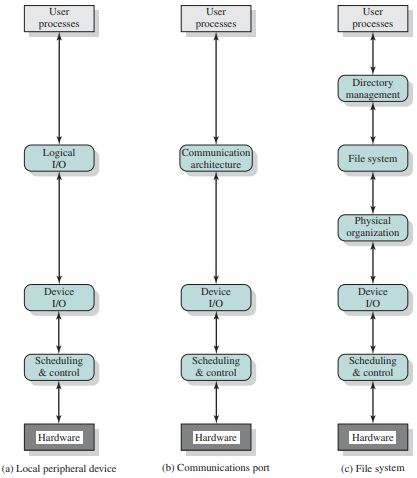
\includegraphics[width=0.5\linewidth]{images/struttura-funzione-io.JPG}
    \caption{Livelli nei dispositivi locali, dispositivi di comunicazione e File System}
    \label{fig:struttura-funzione-io}
\end{figure}

\section{Buffering dell'I/O}
Se un processo emette un comando I/O, viene sospeso in attesa del risultato e quindi viene scambiato prima dell'inizio dell'operazione, il processo viene bloccato in attesa dell'evento I/O e l'operazione di I/O viene bloccata in attesa affinché il processo venga scambiato.
Per evitare questo deadlock\footnote{Indica una situazione in cui due o più processi o azioni si bloccano a vicenda, aspettando che uno esegua una certa azione che serve all'altro e viceversa.}, a volte è conveniente eseguire i trasferimenti di input prima che vengano effettuate le richieste ed eseguire i trasferimenti di output qualche tempo dopo l'esecuzione della richiesta. Questa tecnica è nota come \textit{buffering}.

Prima di discutere i vari approcci al buffering è importante fare una distinzione tra due tipi di dispositivi di I/O: orientati ai blocchi e orientati al flusso. Un dispositivo orientato ai blocchi memorizza le informazioni in blocchi che solitamente hanno dimensioni fisse e i trasferimenti vengono effettuati un blocco alla volta. Un dispositivo orientato al flusso trasferisce i dati in entrata e in uscita come un flusso di byte.

\subsection*{Buffer singolo}
Il tipo più semplice di supporto che il sistema operativo può fornire è il \textit{buffering singolo} (vedi Figura \ref{fig:single-buffer}). Quando un processo utente emette una richiesta I/O, il sistema operativo assegna all'operazione un buffer nella parte di sistema della memoria principale.

\begin{figure}[h]
    \centering
    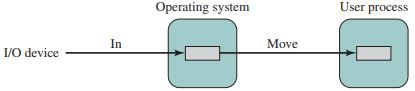
\includegraphics[width=0.5\linewidth]{images/single-buffer.JPG}
    \caption{Buffer singolo}
    \label{fig:single-buffer}
\end{figure}

\begin{itemize}
    \item Per i dispositivi orientati ai blocchi, i trasferimenti di input vengono effettuati nel buffer di sistema e, una volta completato il trasferimento, il processo sposta il blocco nello spazio utente e richiede immediatamente un altro blocco. Questo si chiama lettura anticipata (o input anticipato) e viene fatta perché, nella maggior parte dei casi, i dati vengono acceduti in sequenza.

    Considerazioni simili si applicano all'output orientato ai blocchi. Quando i dati vengono trasmessi a un dispositivo, vengono prima copiati dallo spazio utente nel buffer di sistema, dal quale verranno infine scritti.

    \item Per l'I/O orientato al flusso, lo schema di buffering singolo può essere utilizzato in modo lineare o byte. 
        Il funzionamento a linea è appropriato per i terminali dove l'input e l'output dell'utente sono una riga alla volta, con un ritorno a capo che segnala la fine di una riga. In questo sistema il processo utente viene sospeso durante l'input, in attesa dell'arrivo dell'intera linea e vengono bufferizzate linee intere di input o di output.
        Il funzionamento byte alla volta viene utilizzato quando ogni pressione di un tasto è significativa, e l'interazione tra il sistema operativo e il processo utente segue il modello produttore/consumatore.
\end{itemize}

\subsection*{Buffer doppio}
È possibile ottenere un miglioramento rispetto al buffering singolo assegnando due buffer di sistema all'operazione (vedi Figura \ref{fig:double-buffer}). Un processo ora trasferisce i dati a (o da) un buffer, mentre il sistema operativo svuota (o riempie) l'altro.

\begin{figure}[h]
    \centering
    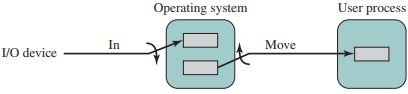
\includegraphics[width=0.5\linewidth]{images/double-buffer.JPG}
    \caption{Buffer doppio}
    \label{fig:double-buffer}
\end{figure}

\subsection*{Buffer circolare}
Se le prestazioni di un particolare processo sono al centro della nostra preoccupazione, allora vorremmo che le operazioni di I/O fossero in grado di tenere il passo con il processo e il doppio buffering potrebbe essere inadeguato.
Quando vengono utilizzati più di due buffer, l'insieme dei buffer viene esso stesso definito \textit{buffer circolare} (vedi Figura \ref{fig:circular-buffer}), dove ogni singolo buffer rappresenta un'unità nel buffer circolare.

\begin{figure}[h]
    \centering
    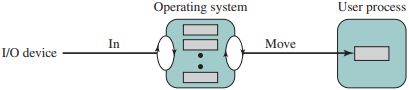
\includegraphics[width=0.5\linewidth]{images/circular-buffer.JPG}
    \caption{Buffer circolare}
    \label{fig:circular-buffer}
\end{figure}

\subsection*{L'utilità del buffering}
Il buffering smussa i picchi di richieste di I/O, tuttavia, nessuna quantità di buffering consentirà a un dispositivo I/O di tenere il passo con un processo quando la domanda media è maggiore di quella che il dispositivo può soddisfare. Tuttavia, in un ambiente di multiprogrammazione, quando sono presenti una varietà di attività di I/O e di processi da servire, il buffering è uno strumento che può aumentare l'efficienza del sistema operativo e le prestazioni dei singoli processi.

\section{Scheduling del disco}
Un disco HDD (Hard Drive Disk) è composto da tracce (corone circolari) e da settori (partizioni di una traccia), vedi Figura \ref{fig:disk}. 
\begin{figure}[h]
    \centering
    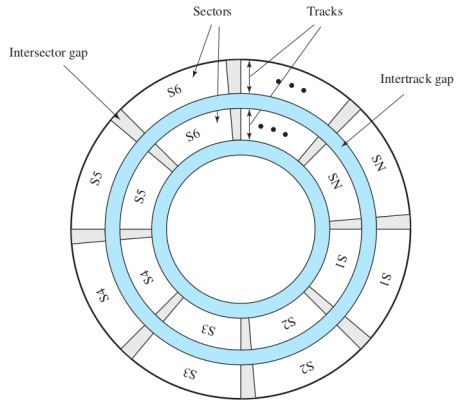
\includegraphics[width=0.5\linewidth]{images/disk.JPG}
    \caption{Disco}
    \label{fig:disk}
\end{figure}
Per leggere o scrivere su disco bisogna selezionare una traccia tramite una testina e, sulla traccia scelta, individuare il giusto settore. Per selezionare una traccia bisogna spostare una testina, se il disco ha testine mobili oppure selezionarla, se il disco ha testine fisse, per selezionare un settore, invece, bisogna aspettare che il disco ruoti.

\subsection*{Prestazioni del disco}
Un diagramma temporale generale del trasferimento I/O del disco è mostrato nella Figura \ref{fig:disk-time}.
\begin{figure}[h]
    \centering
    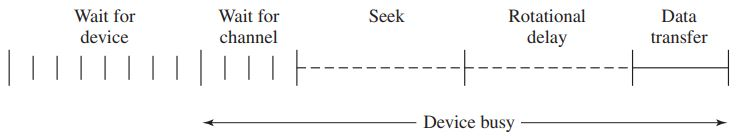
\includegraphics[width=0.7\linewidth]{images/disk-time.JPG}
    \caption{Diagramma temporale su disco}
    \label{fig:disk-time}
\end{figure}
In un primo momento il sistema operativo deve attendere che il disco sia libero (\verb|Wait for device|) e selezionare un suo canale (\verb|Wait for channel|). Una volta fatto ciò, quando l'unità disco è in funzione, il disco ruota a velocità costante e la testina deve essere posizionata sulla traccia desiderata e all'inizio del settore desiderato su quella traccia. Il tempo necessario per posizionare la testa sulla traccia è noto come tempo di ricerca (\verb|Seek|) e una volta selezionata la traccia, il controller del disco attende che il settore appropriato ruoti per allinearsi con la testina. Il tempo impiegato dall'inizio del settore per raggiungere la testa è noto come ritardo rotazionale (\verb|Rotational delay|). La somma del tempo di ricerca, se presente, e del ritardo di rotazione è uguale al tempo di accesso, ovvero il tempo necessario per mettersi in posizione per leggere o scrivere. Una volta che la testina è in posizione, l'operazione di lettura o scrittura viene poi eseguita man mano che il settore si sposta sotto la testina, questa è la parte dell'operazione relativa al trasferimento dei dati.

\subsection*{Politiche di scheduling per il disco}
Anche per il disco sono stati pensati diversi algoritmi per rendere più efficiente l'operazione di lettura o scrittura.

\begin{Example}{Algoritmi di scheduling per il disco}{}
    \textit{Supponiamo di avere un disco con 200 tracce con la testina del disco inizialmente posizionata sulla traccia 100. Le tracce richieste, nell'ordine ricevuto dallo scheduler del disco, sono:}
    \begin{equation*}
        55,\mbox{ }58,\mbox{ }39,\mbox{ }18,\mbox{ }90,\mbox{ }160,\mbox{ }150,\mbox{ }38,\mbox{ }184  
    \end{equation*}
    \begin{itemize}
        \item Con il \textit{FIFO} (First In First Out) le richieste vengono servite in modo sequenziale e la testina si muove continuamente avanti e dietro, se ci sono molti processi in esecuzione, le prestazioni sono simili ad uno scheduling random;

         \begin{minipage}{\textwidth}
            \centering
            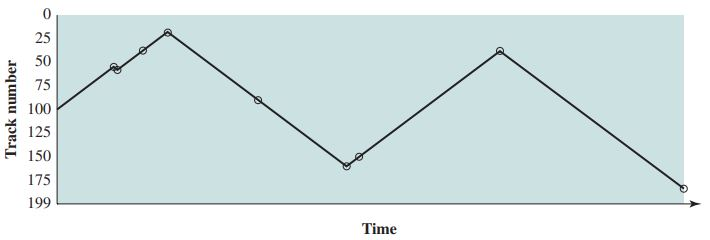
\includegraphics[width=0.5\linewidth]{images/esempio-fifo-disk.JPG}
        \end{minipage}

        \item Con il SSTF (Shortest Service Time First) si sceglie la richiesta che minimizza il movimento della testina dalla posizione attuale. Naturalmente, scegliere sempre il tempo di ricerca minimo non garantisce che il tempo di ricerca medio su un certo numero di movimenti del braccio sia minimo. Inoltre c'è la possibilità di ricorrere nella starvation delle richieste perché potrebbero arrivare continuamente richieste più vicine;

        \begin{minipage}{\textwidth}
            \centering
            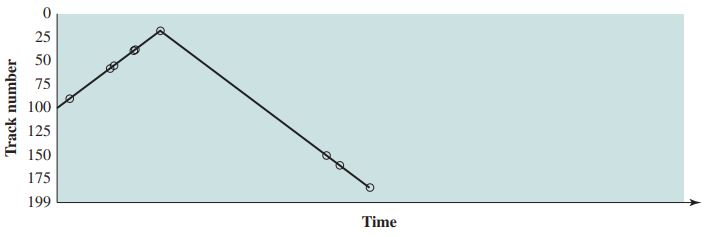
\includegraphics[width=0.5\linewidth]{images/esempio-sstf-disk.JPG}
        \end{minipage}
    
        \item Con lo \textit{SCAN} si scelgono le richieste in modo tale che il braccio si muova sempre in un verso, e poi torni indietro. Questo sistema elimina la starvation delle richieste, in quanto possono accumularsi solo in un verso e successivamente vengono terminate, ma è poco equo perché favorisce le richieste vicino ai bordi o quelle appena arrivate. Questi problemi possono essere risolti con il C-SCAN e F-SCAN.

        \begin{minipage}{\textwidth}
            \centering
            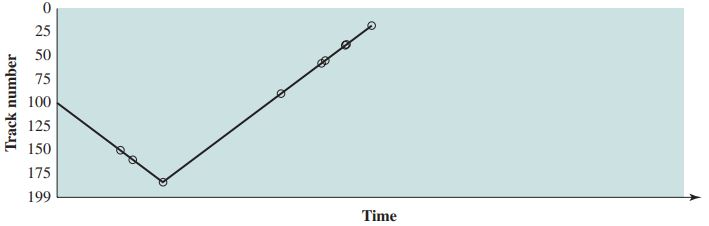
\includegraphics[width=0.5\linewidth]{images/esempio-scan-disk.JPG}
        \end{minipage}

        \item Con il \textit{C-SCAN} si servono le richieste solo in una direzione, in questo modo i bordi non sono più visitati 2 volte in poco tempo;

        \begin{minipage}{\textwidth}
            \centering
            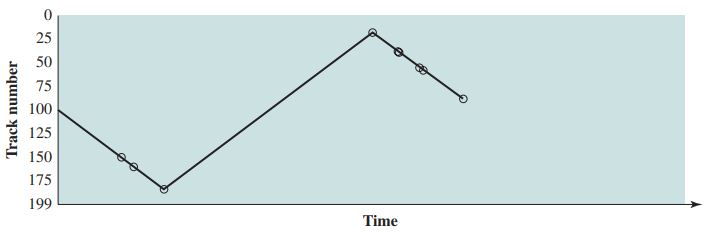
\includegraphics[width=0.5\linewidth]{images/esempio-cscan-disk.JPG}
        \end{minipage}
        
        \item Con l'\textit{F-SCAN} si utilizzano due code Front (F) e Rear (R) e, mentre SCAN serve la coda F, ogni nuova richiesta è aggiunta alla coda R, quando SCAN finisce di servire F, si scambiano F ed R. Ogni nuova richiesta deve aspettare che tutte le precedenti vengano servite e quindi le richieste vecchie non perdono di priorità;

        \item Si può generalizzare l'F-SCAN con l'\textit{N-step-SCAN} dove si accodano le richieste nella coda i-esima finché non si riempie, poi si passa alla $(i + 1)\mod{N}$.
    \end{itemize}
\end{Example}

\section{Cache del disco}
La cache del disco è un buffer in memoria principale che contiene una copia di alcuni settori del disco. Quando si fa una richiesta di I/O per dati che si trovano su un certo settore, si vede prima se tale settore è nella cache, se non è presente viene anche copiato nella cache. 

Ci sono svariati metodi per gestire il rimpiazzo di un settore nella cache piena: un algoritmo comunemente utilizzato è LRU, dove si sostituisce il blocco che è rimasto nella cache da più tempo senza referenze. La cache viene puntata da uno “stack” di puntatori e il settore riferito più di frequente è alla cima dello stack. Quindi, ogni volta che un settore viene referenziato o copiato nella cache, il suo puntatore viene portato in cima allo stack. Un'altra possibilità è LFU che sostituisce il settore con il minor numero di riferimenti. LFU potrebbe essere implementato associando un contatore a ciascun blocco e quando viene introdotto un blocco, gli viene assegnato un conteggio pari a 1. Ad ogni riferimento il suo conteggio viene incrementato di 1 e, quando è richiesta la sostituzione, viene selezionato il blocco con il conteggio più piccolo. Un semplice algoritmo LFU presenta il seguente problema: è possibile che, a causa della località, un settore viene acceduto svariate volte di fila, al termine di tale intervallo, il conteggio dei riferimenti potrebbe avere un valore abbastanza alto quando in realtà il settore andrebbe sostituito. L'idea è quella di combinare LRU e LFU con uno “stack” di puntatori diviso in due parti una nuova e una vecchia ed operare come segue (vedi Figura \ref{fig:lru-lfu-disk}):
\begin{enumerate}
    \item Quando un blocco viene referenziato per la prima volta (cache miss), lo si sposta all'inizio della nuova sezione con un conteggio pari a 1;
    \item Se il blocco viene referenziato quando è nella nuova sezione il suo conteggio dei riferimenti non viene incrementato; ciò fa sì che i conteggi per i blocchi a cui viene fatto ripetutamente riferimento rimangano invariati;
    \item Quando il blocco passa alla vecchia sezione per scorrimento (quando un blocco vecchio viene riferito e diventa nuovo, spinge l’ultimo dei nuovi a diventare primo dei vecchi) e viene referenziato, ritorna alla cima dello stack con il conteggio incrementato di 1.
\end{enumerate}

\begin{figure}[h]
    \centering
    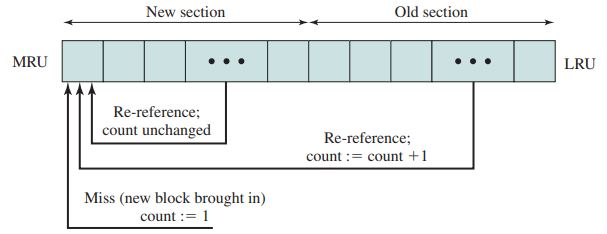
\includegraphics[width=0.7\linewidth]{images/lru-lfu-disk.JPG}
    \caption{Sostituzione di blocchi basata sulla frequenza con due sezioni}
    \label{fig:lru-lfu-disk}
\end{figure}

C'è ancora un problema in questo sistema: se un nuovo blocco, che è passato alla vecchia sezione, non viene ri-referenziato abbastanza rapidamente, è molto probabile che venga sostituito perché ha necessariamente il conteggio di riferimenti più piccolo tra quelli che sono nella vecchia sezione. Per risolvere questo problema si può dividere lo stack in tre sezioni: nuova, media e vecchia (vedi Figura \ref{fig:rimpiazzamento-due-sezioni}). Sia nella parte nuova che in quella media non possono essere effettuati i rimpiazzamenti, con la differenza che nella media e nella vecchia sezione i contatori vengono incrementati.

\begin{figure}[h]
    \centering
    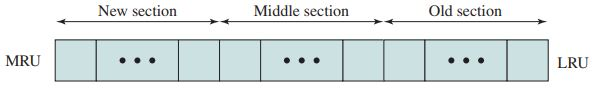
\includegraphics[width=0.7\linewidth]{images/rimpiazzamento-due-sezioni.JPG}
    \caption{Sostituzione di blocchi basata sulla frequenza con tre sezioni}
    \label{fig:rimpiazzamento-due-sezioni}
\end{figure}

\section{RAID}
Con i dischi \textit{RAID} (Redundant Array of Independent Disks) si hanno a disposizione più dischi fisici che si possono trattare separatamente. Su Windows, per esempio, si mostrano esplicitamente dischi diversi, con etichette diverse (C, D...), in Linux, alcuni files/directory sono memorizzati su un disco, altri su un altro e, tramite LVM (Logical Volume Mananger), l’utente non deve occuparsi di decidere dove salvare i file.
Un'altra possibilità è considerare diversi dischi fisici come un unico disco.

L’LVM va bene per pochi dischi, ed in generale non si è interessati alla ridondanza, ovvero non si occupa di memorizzare dati uguali su diversi dispositivi come backup. Con i dischi RAID, invece, non solo si risolve questo problema ma si riesce anche a velocizzare alcune operazioni, grazie ad una gerarchia a più livelli.

\subsection*{RAID livello 0}
Il livello più basso della gerarchia di RAID è quello 0 (vedi Figura \ref{fig:raid0}), dove i dischi vengono divisi in \textit{strip}, a loro volta sono divisi in settori, un insieme di strips sui vari dischi (una riga) si chiama \textit{stripe}. In questo livello non c'è ridondanza dei dati ma si utilizza la parallelizzazione su più strips per maggiore efficienza nell'accesso.

\begin{figure}[h]
    \centering
    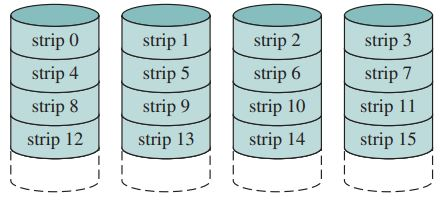
\includegraphics[width=0.5\linewidth]{images/raid0.JPG}
    \caption{Raid livello 0}
    \label{fig:raid0}
\end{figure}

\subsection*{RAID livello 1}
Nel RAID livello 1, metà della memoria di archiviazione viene utilizzata per duplicare ogni disco (vedi Figura \ref{fig:raid1}). In questo modo se si rompe un disco si ha un recupero sicuro dei dati.

\begin{figure}[h]
    \centering
    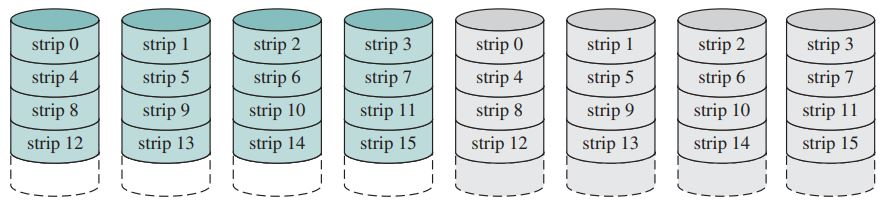
\includegraphics[width=0.5\linewidth]{images/raid1.JPG}
    \caption{Raid livello 1}
    \label{fig:raid1}
\end{figure}

\subsection*{RAID livello 2}
Nella maggior parte dei casi, un disco non si rompe per intero, ma al più una sua parte o qualche suo bit. Per tanto è inutile replicare l’intera informazione, è più efficiente utilizzare dei codici particolari, per esempio, il codice di Hamming che può correggere errori su singoli bit. In questo modo non saranno utilizzati $N$ dischi di overhead, ma ne serviranno il giusto numero per memorizzare il codice scelto (vedi Figura \ref{fig:raid2}).

\begin{figure}[h]
    \centering
    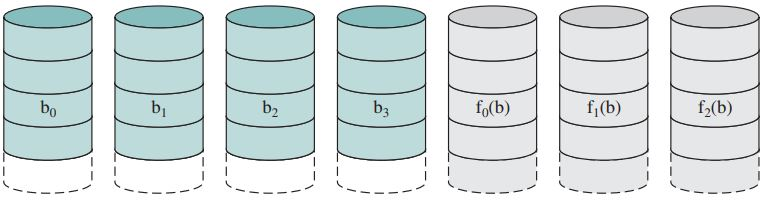
\includegraphics[width=0.5\linewidth]{images/raid2.JPG}
    \caption{Raid livello 2}
    \label{fig:raid2}
\end{figure}

\subsection*{RAID livello 3}
Nel RAID livello 3, viene utilizzato un solo disco di overhead (vedi Figura \ref{fig:raid3}). In questo livello ogni strip è considerato come un byte e, sul disco di overhead, viene memorizzato, per ogni bit, la parità dei bit che hanno la stessa posizione, in questo modo resta possibile recuperare i dati quando fallisce un unico disco.

\begin{figure}[h]
    \centering
    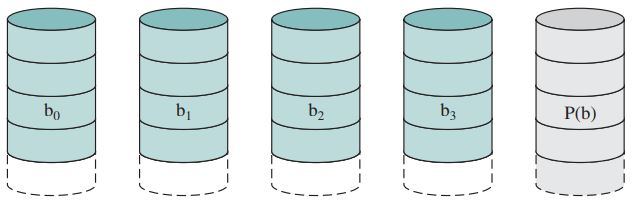
\includegraphics[width=0.5\linewidth]{images/raid3.JPG}
    \caption{Raid livello 3}
    \label{fig:raid3}
\end{figure}

\subsection*{RAID livello 4}
In questo livello si hanno le stesse caratteristiche del RAID livello 3, ma con la differenza che ogni strip è un “blocco”, potenzialmente grande, recuperabile in caso di fallimento di un unico disco (vedi Figura \ref{fig:raid4}).

\begin{figure}[h]
    \centering
    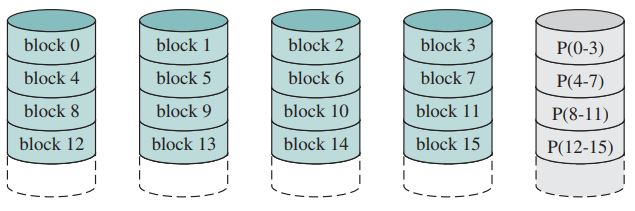
\includegraphics[width=0.5\linewidth]{images/raid4.JPG}
    \caption{Raid livello 4}
    \label{fig:raid4}
\end{figure}

\subsection*{RAID livello 5}
Nel livello 5, le informazioni di parità non sono tutte su un unico disco (vedi Figura \ref{fig:raid5}). In questo modo si evita il collo di bottiglia del disco di parità e non c'è un disco “privilegiato” che salva le informazioni.

\begin{figure}[h]
    \centering
    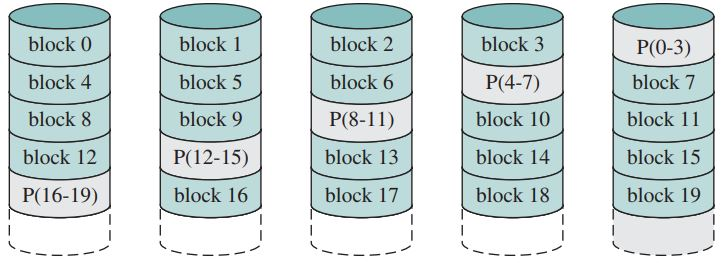
\includegraphics[width=0.5\linewidth]{images/raid5.JPG}
    \caption{Raid livello 5}
    \label{fig:raid5}
\end{figure}

\subsection*{RAID livello 6}
Il RAID livello 6 è come il livello 5, ma con 2 dischi di parità indipendenti in modo da poter recuperare anche 2 fallimenti di disco (vedi Figura \ref{fig:raid6}).

\begin{figure}[h]
    \centering
    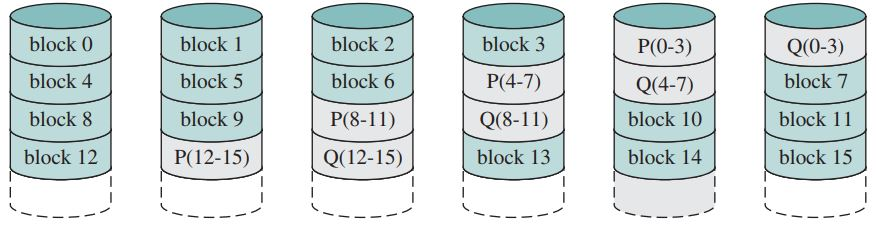
\includegraphics[width=0.5\linewidth]{images/raid6.JPG}
    \caption{Raid livello 6}
    \label{fig:raid6}
\end{figure}

Da notare che se viene effettuata un’operazione sul RAID, tutti i dischi effettuano in sincrono quell'operazione, e un’operazione sul RAID è un’operazione su un sottoinsieme dei suoi dischi, questo permette il completamento in parallelo di richieste I/O distinte.

\section{I/O in Linux}
In Linux si ha un'unica page cache per tutti i trasferimenti tra disco e memoria, compresi quelli dovuti alla gestione della memoria virtuale, questo permette di condensare le scritture e di sfruttare la località dei riferimenti per risparmiare accessi su disco. Viene effettuata una scrittura su disco solo quando è rimasta poca memoria o quando l'età delle pagine “sporche” va sopra una certa soglia. Inoltre non c'è una politica di replacement separata, ma è la stessa usata per il rimpiazzamento delle pagine.